\chapter{Controller Design (worksheets)}\label{ch:Controller}
We now have a linearized model for the entire system, where system estimation has been done. Read the other section concerning this procedure. \newpar 
The model of the system is:
\begin{equation}
G=\frac{275.9}{s(s-5.96)(s+17.6)} \label{kkk}
\end{equation}
We have chosen to make a cascade controller of two loops. The controller in the inner loop is to have the voltage as output and angular velocity as input. The controller in the outer loop is to have angular velocity as output and angle as input.\\
This is illustrated in the block diagram of the cascade control feedback loop. 
\begin{figure}[H]
	\centering
	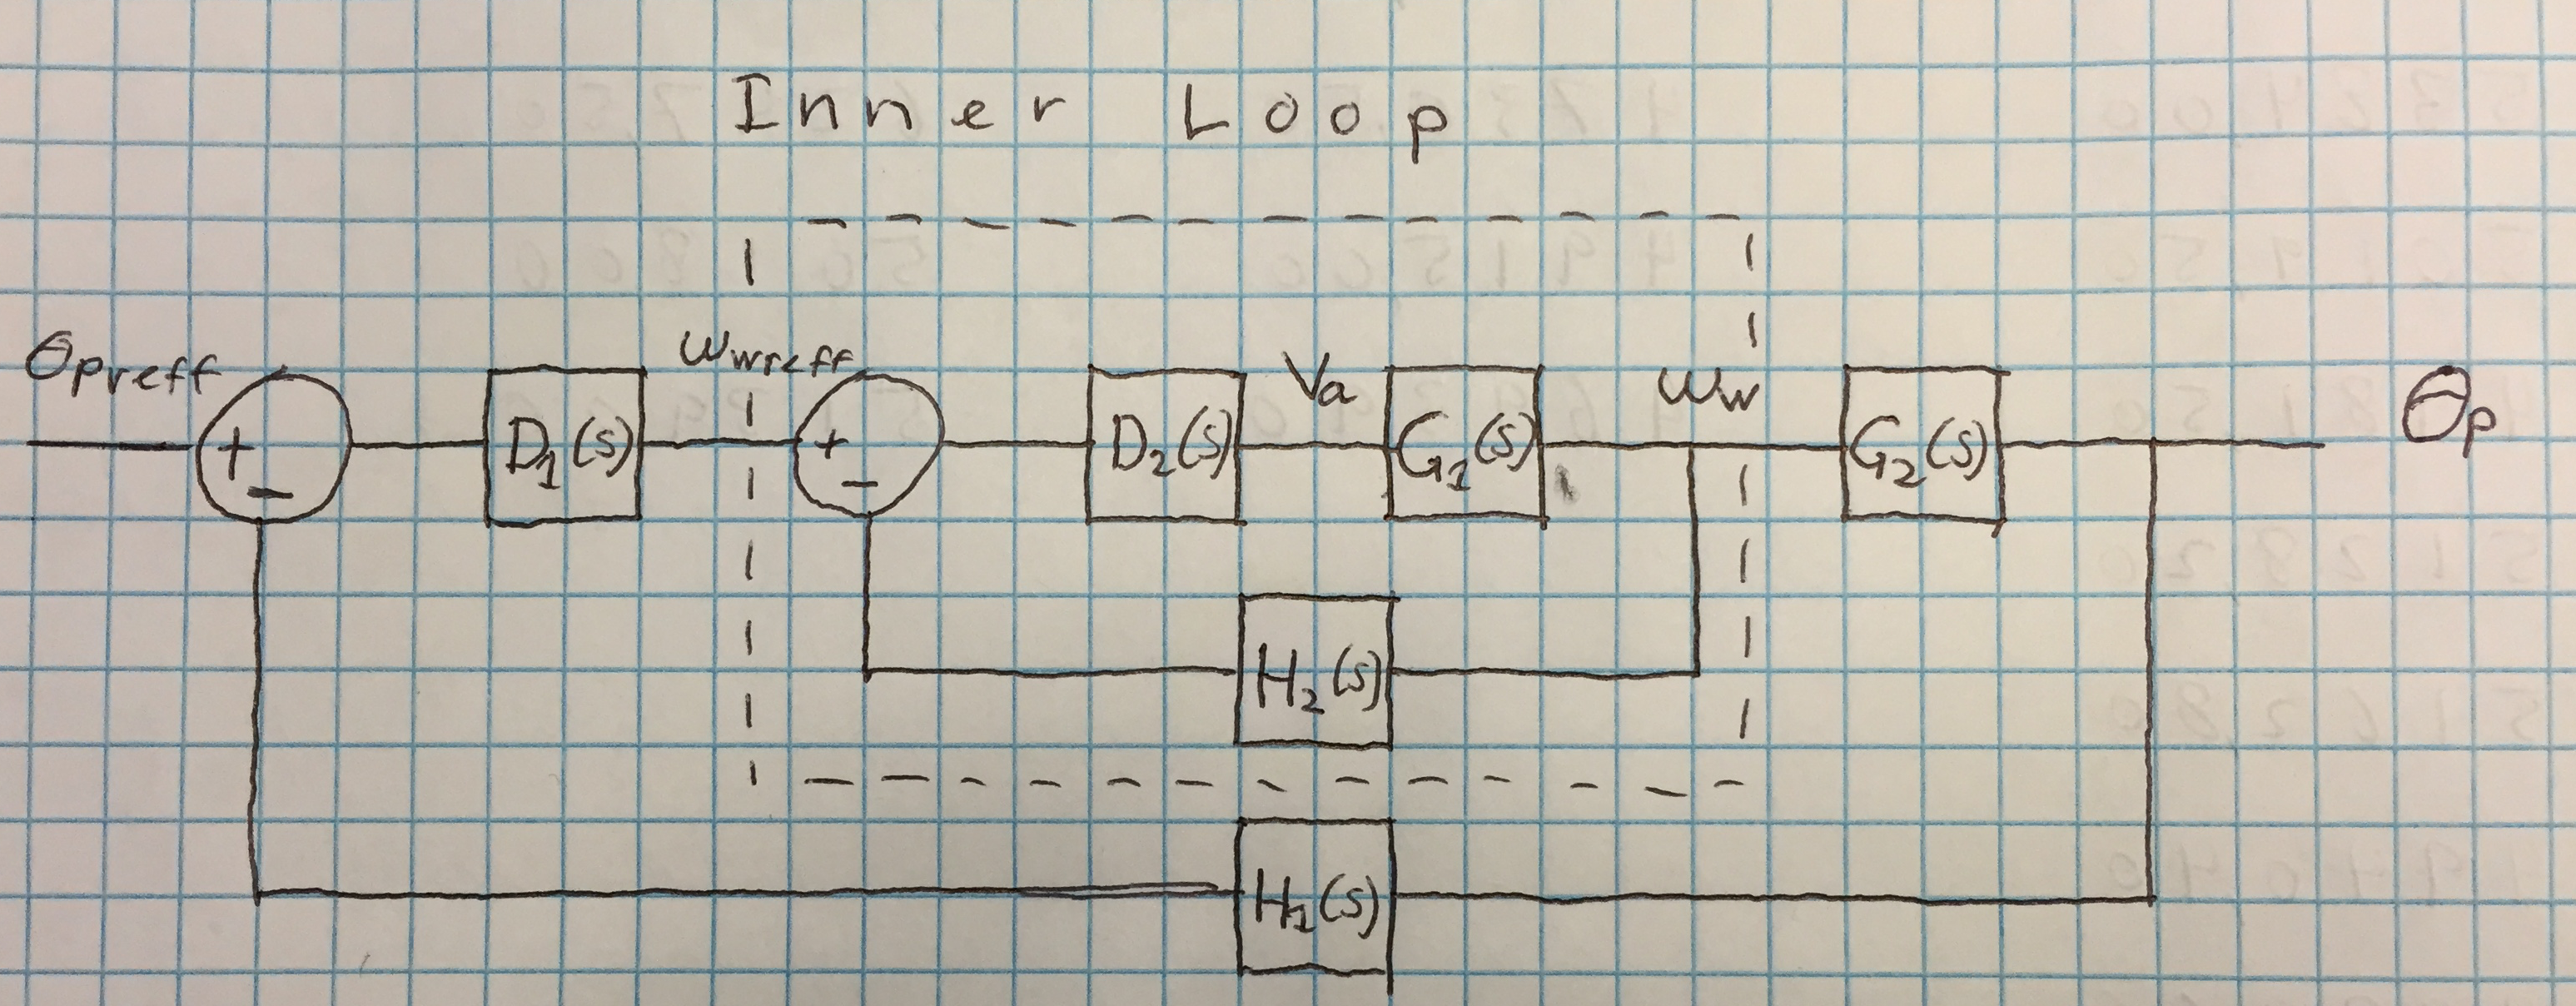
\includegraphics[width=0.7\textwidth]{figures/cascadecontroller.png}
	\caption{Cascade control loop.}
\end{figure}
We know from our modelling that there is a single stable pole in the motor and wheels model, and that the pole is placed further out in the LHP that the poles in the model for the inverted pendulum is. The gain of the motor and wheels model is known as 4.00. This was found by measuring the velocity of the wheel at full supply voltage (s = 0). From this the model for the motor and wheel can be determined as shown here:
\begin{equation}
\frac{G}{s+17.6}=4.00\Rightarrow 70.4
\end{equation}

Since the whole model covers the model for the inverted pendulum and the motors and wheels, the model for the inverted pendulum can now be determined. The two remaining poles is from the inverted pendulum, which seems right as one of the poles is in the RHP. The gain of the inverted pendulum can be determined as the gain of the complete model divided with the gain of the motor and wheels model. This yields the two separated models:
\begin{align}
G_2&=\frac{70.4}{s+17.6}\\
G_1&=\frac{3.92}{s(s-5.96)}
\end{align}







%The system model can be divided into two plants, as seen in the block diagram. 
%We take our starting point at the motor and wheels model:
%\begin{equation}
%G_{mw}=\frac{\omega_m}{Va}=\frac{49}{s+9.214}
%\end{equation}
%
%\begin{align}
%&\frac{\omega_p}{\omega_w}=\frac{b}{s-5.96}\\
%&\omega_p(j\omega)=\frac{b}{-5.96}\cdot \omega_w(j\omega)
%\end{align}
%
%\begin{equation}
%\frac{\omega_m}{Va}\approx \frac{\frac{1.1}{r_w}}{5}
%\end{equation}
%\begin{where}
%\va{$r_w$}{is the radius of a wheel}{m}
%\end{where}
%Note, that s is equal to zero in the above expression. \newpar
%Now we can determine the two transfer functions. 
%\begin{align}
%G_2&=\frac{70.4}{s+17.6}\\
%G_1&=\frac{3.92}{s(s-5.96)}
%\end{align}
When we look at the transfer function of the entire system, \autoref{kkk}, we see that we have a zero pole, a negative and a positive pole. \newpar

As the inner loop, $G_2$ already is a stable system, and it is the inner loop, it has to be fast, to allow it to be seen as 1 for the outer loop. The inner loop is controlled by a P controller. Its gain is set to $K_p=10$, as this gives a reasonable step response. \newpar
The outer loop, $G_1$ is unstable. We want to move the RHP pole into the LHP, to ensure a stable system. We have decided to design a lead controller as the phase margin of the system is -83.7 degress. We want a phase margin of 50 degrees. \\
Phaselift can be determined:
\begin{equation}
PL=180+83.7-130=134
\end{equation}
The phase has to be lifted 134 degrees. From this we see, that a single lead controller will not be able to lift the phase sufficiently. Therefore a double lead controller is to be designed. 
The phase lift done by each lead controller. 
\begin{equation}
PL_1=\frac{PL}{2}=\frac{134}{2}=67
\end{equation}
We know from formulas in our control book the following deriviation. The controller is as following:
\begin{equation}
C=K\frac{\tau s +1}{\alpha \tau s +1}
\end{equation}
Where $\alpha$ is smaller than one. 
Alpha can be found: 
\begin{equation}
\alpha=\frac{1-\sin(PL_1)}{1+\sin(PL_1)}=0.0414
\end{equation}
The risetime can be found from the decided settling time. Settlingtime can be expressed as:
\begin{equation}
t_s=\frac{-ln(x)}{\epsilon \omega_w}=\frac{4.6}{\epsilon \omega_w}
\end{equation}
where x=0.01. Note that 3 is the settling time decided by the group. \\
Together with the following expression, $\omega_n$ can be found.
\begin{align}
\epsilon\approx \frac{PM}{100}=\frac{50}{100}=0.5
\end{align}
From this we can determine $\omega_n$:
\begin{equation}
\frac{4.6}{0.5\cdot \omega_n}=3 \Rightarrow \omega_n=3
\end{equation}
When we have $\omega_n$ we have a formular to determine the risetime:
\begin{equation}
t_r=\frac{1.8}{\omega_n}=\frac{1.8}{3}=0.587
\end{equation}
From the above we can now determine the $\tau$ factor:
\begin{equation}
\omega_{bw}=4.2=\frac{1}{\tau \sqrt{\alpha}}\Rightarrow \tau=1.17
\end{equation}
 
The controller is now:
\begin{equation}
C=K\frac{1.17s +1}{0.0414\cdot 1.17s +1}
\end{equation}
We choose K to be 1, as we see, that this will make the positive pole negative. 
The final controller is:
\begin{equation}
C= (\frac{1+0.97s}{1+0.04s})^2
\end{equation}





\section{Implemented controller}

The following transfer function corresponds to the implemented controller. It has been made based on the calculation of the above.
\begin{align}
H(z)=\dfrac{2,64-2,24 \cdot z^{-1}}{1-z^{-1}}
\end{align}

The following equation (bilinear transformation) is used to get from $Z$-domain to $S$-domain (inverse $Z$ transform). Here, $T_{d}=10$ms.
\begin{align}
z=\dfrac{1+ \dfrac{T_{d}}{2} \cdot s}{1-\dfrac{T_{d}}{2} \cdot s}
\end{align}

By replacing the z-term with the expression of the above, the result obtained is:
\begin{align}
H(s) &= \dfrac{2,64- \left( \dfrac{1- \dfrac{T_{d}}{2} \cdot s}{1+ \dfrac{T_{d}}{2} \cdot s} \right) \cdot 2,24}{1- \left( \dfrac{1- \dfrac{T_{d}}{2} \cdot s}{1+ \dfrac{T_{d}}{2} \cdot s} \right) }\\
&= \dfrac{ \left( 1+ \dfrac{T_{d}}{2} \cdot s \right) \cdot 2,64- \left( 1- \dfrac{T_{d}}{2} \cdot s \right) \cdot 2,24}{T_{d} \cdot s}\\
&= \dfrac{0,4}{T_{d} \cdot s} + 2,44\\
&= \dfrac{40+2,44 \cdot s}{s}
\end{align}

It is possible to identify an integrator in the above expression's denominator ($\dfrac{1}{s}$ term).

There is also a zero in the numerator. By solving the $40+2,44 \cdot s=0$, the solution obtained is $s=-16.3934$.